\section{Introduction}
\quad \quad Vulnerability scanners have the unique property of allowing automated scans against a certain system, 
network, or application. This extends to web applications as well, and there are a variety of different types of scanners 
that have both comparable and differing functionality. This paper will primarily focus on a Web Application
scanner called Wapiti, but other tools will be discussed as well in order to compare functionality. The rest of
the article is structured as follows. The \hyperref[sec:motive]{next section} gives the motivation as to why
Vulnerability Scanners are important. \hyperref[sec:tools]{Section 3} will contain discussion around Wapiti and other tools similar to it.
\hyperref[sec:demo]{Section 4} will show a demo of how Wapiti can be used to scan a web application. 
\hyperref[sec:opts]{Section 5} will go over some of the useful commands that Wapiti can offer, and then \hyperref[sec:conclude]{Section 6} will conclude the paper.
\section{Motivation} \label{sec:motive}
\quad \quad Studying vulnerability scanners is important because they allow us to validate the security of our applications. 
For the purpose of this paper, we are more interested in accessing the validity of online web applications. Making sure 
our web applications are secure is pivotal due to the sheer load of requests and interactions users make with websites
every day. It is in the best interest of companies around the world to keep their sites both online and secure in the hopes
of retaining customers. Even just one security breach or outage caused by an attack can turn a customer away forever, 
therefore it is ideal for a business to keep their applications online as much as possible. These attacks can be prevented ahead of time
by using vulnerability scanners to detect any defects within a web application, and from the output given by a tool
a plan can be made to correct whatever vulnerability is present. For this reason it is both necessary to know how and when 
to use a given tool.
\section{Tool Analysis} \label{sec:tools}
\quad \quad The goal of this section is to describe the features and functionality of the Wapiti tool, as well as a couple of
similar tools for comparison.
\subsection{Wapiti}
\quad \quad Wapiti is an open source web application scanner that specializes in black-box scans, written in python. According 
to its official website, it does not study the source code of a site, but instead \say{[crawls] the webpages of the 
deployed webapp, looking for scripts and forms where it can inject data}[1]. It has a variety of 
modules that can detect vulnerabilities in areas such as SQL Injection, Cross Site Scripting (XSS), and in recent updates 
Log4Shell vulnerability detection has even been added. It has more than just these, and they can be easily be changed and customized 
through the use of flags. After the completion of the tool, it will generate a report in either json, html, txt, 
or xml format depending on the user's choice. In this report it will tell you the number of vulnerabilities found for each 
module used, descriptions of the types of scans used, and even some recommended solutions to try and fix 
some of the vulnerabilities.
\subsection{Vega}
\quad \quad Vega is another open source web application scanner. Like Wapiti it also has modules that can scan for SQL Injection and 
Cross Site Scripting vulnerabilities. It \say{works on Linux, OSX and Windows platform since its detection modules are written in 
JavaScript and additional modules can be developed by using its API's}[4]. The main differences between
Wapiti and Vega come from the fact that Vega has its own Graphical User Interface (GUI) and Application Programming Interface (API) infrastructure. Due to this, Vega is a bit more user
friendly out the box, and if one is knowledgeable enough to make their own JavaScript detection modules that option is 
available to them. Wapiti has the advantage of still receiving updates to the tool as recent
as February 2022, while Vega hasn't been updated since June 2016 according to its last github commit. Both tools have 
their own strengths though, and I would say Vega specializes in its user friendliness and customizability.
\subsection{w3af}
\quad \quad The final tool being discussed in this paper is w3af, which like Wapiti is also written in python. It has both
a GUI and Shell interface, and like the previous two tools it features a plethora of different modules for a user to scan 
with. It also advertises itself as being \say{easy to use and extend}[3], which could be helpful for any developers looking to 
create their own types of scans. It looks very convenient for doing repeated testing, as different types of scanning configurations
can be saved for later use.
\subsection{Concluding Tool Discussion}
\quad \quad Overall all three of these tools are similar in terms of the types of scans they can apply to web applications. Wapiti is an intuitive command line tool that 
has a variety of scanning modules that are still updated to this day. 
Vega on the other hand hasn't had recent updates like Wapiti, but is still powerful and features a nice graphical 
interface. A good compromise between the two is w3af, which features both a command line and graphical interface, as well
as a large variety of scanning modules. The next section will give an in depth demo of how to use Wapiti.
\section{Wapiti Demo} \label{sec:demo}
\subsection{Experimental Setup}
In order to setup the experiment I used a Kali 2021 (Version 5.10.0) virtual machine with an Open Web Application Security Project Broken Web Applications (OWASPBWA)
virtual machine (Version 2.6.32) to serve as a target for the experiment. Both machines were run using 
Oracle VM Virtual Box, and both were also set to Host-Only Adapter mode to ensure a safe environment.
Wapiti comes preinstalled with Kali Linux, so it wasn't necessary to do any installation.
\subsection{Launching a scan}
To start first make sure that your OWASPBWA virtual machine is launched. If you don't know the IP Address
of the OWASPBWA system, you can use the ifconfig command inside the terminal to get the address. Once you know the address 
and your OWASPBWA machine is on, launch the Kali virtual machine and open the command prompt. For this test we are going to 
use the default scanning tests provided by Wapiti (If you want to learn more about some helpful Wapiti commands, continue
to section 5). In order to do this we are going to use the following command:
\begin{verbatim}
wapiti -u [SITE TO SCAN]
\end{verbatim}
In this case the site to scan is going to be inside of the OWASPBWA virtual machine. It has a variety of different
web applications on it that are intentionally left vulnerable. For this test we are going to target the site known
as the bodgeit store, which according to the developer's github page contains significant vulnerabilities in \say{Cross Site
Scripting, SQL Injection, Hidden Content}[5], as well as other vulnerabilities. So in order to reach this webpage,
it is only necessary to provide:
\begin{verbatim}
http:// + TARGET IP ADDRESS + /bodgeit
\end{verbatim} 
If we were targeting an actual webpage it wouldn't be necessary to deal with finding the site on an ip address, but since this test
uses two machines in Host-Only mode this is necessary to provide the correct path to the webpage. Here is an example of what the full
command will look like in the terminal:
\begin{center}
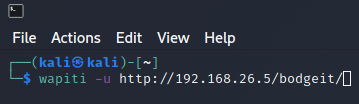
\includegraphics[width=.5\textwidth]{default_cmd.png}
Table 1: Default command for Wapiti
\end{center}
When this command is run, it will start all the default scans provided by Wapiti. This is excluding some of the other modules, but they can
be included if the user desires (discussed in next section). Once this command starts running, the tool will start going through all of the 
different modules included. After that the tool will finish, and it will output a report of what the tool found in html format by default.
\begin{center}
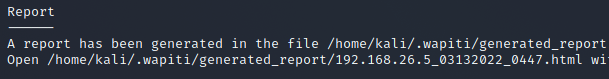
\includegraphics[width=.55\textwidth]{report_final.png}
Table 2: Wapiti report location
\end{center}
The report is sent by default to a folder in the home directory, but the tool will let you know where the file was sent.
In this report, it first starts by providing a summary of how many vulnerabilities of each type were found by the scanner.
\begin{center}
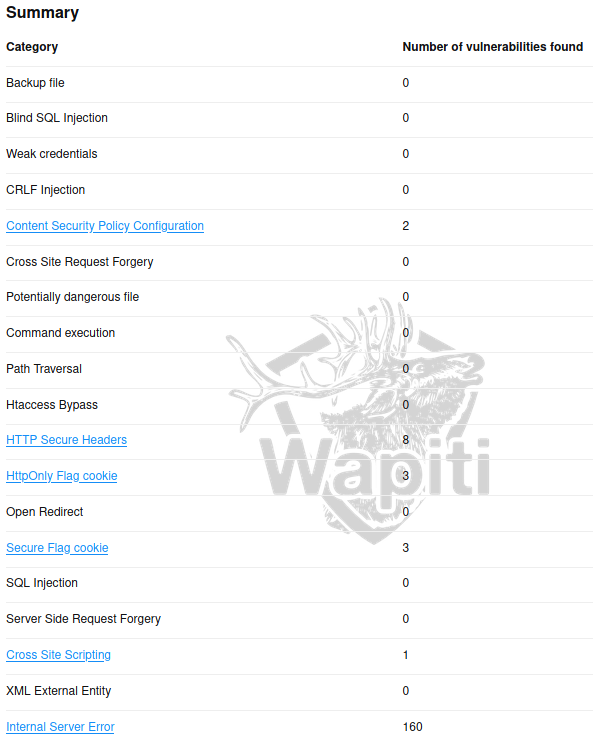
\includegraphics[width=.5\textwidth]{report_sum.png}
Table 3: Wapiti report summary
\end{center}
If a vulnerability was found, you can look into the details and see description of the vulnerability, and if applicable the HTTP request or 
cURL command used by the tool.
\begin{center}
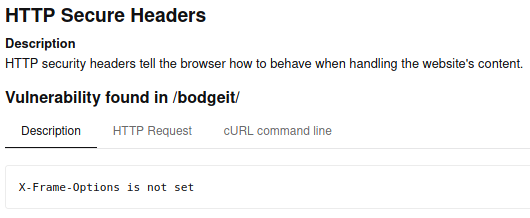
\includegraphics[width=.5\textwidth]{ex_error.png}
Table 4: Wapiti vulnerability found
\end{center}
After going through all of the vulnerabilities listed in the report, this final line will give some tips if it can on how to fix any of the vulnerabilities. 
It will also list any references it thinks it would be helpful.
\begin{center}
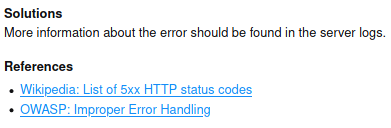
\includegraphics[width=.5\textwidth]{help.png}
Table 5: Wapiti helpful tips
\end{center}
Using Wapiti with the default options is a good way to scan a web application without too much difficulty. Wapiti also has 
a variety of different flags and options available to it though, and those will be discussed in the next section.
\section{Wapiti options}\label{sec:opts}
Wapiti has a variety of different options that give users more customizability when launching a scan. The following subsections will list some of the flags that
I found to be the most important when I read through the manual.
\subsection{The --scope flag}
With the scope flag, the user can define how deep the scanner should go. By default the \say{url} value is used, which only scans the base url provided to the tool. If
\say{folder} in inputted into the tool instead, it \say{will scan and attack every URL starting with the base URL value}[6]. If \say{domain} is passed in, it 
\say{will scan and attack every URL whose domain name match the one from the base URL}[6]. Finally, and most dangerous, the \say{punk} option will scan every URL that it 
can find while the tool is running. While these could be useful, they should be used sparingly as if not careful the tool could scan a webpage that it is not authorized to scan.
\subsection{The -m flag (modules)}
Wapiti has many different modules that it can use for scanning purposes, many of which it uses by default. If a user wants to be more selective with what modules are
used, they can call the -m flag with the modules they want separated by commas. The command --list-modules can also be used to see what the current modules available are.
\subsection{The -a flag}
The -a flag or --auth-type is a flag to set the login credentials of a particular site if needed for a scan. They should be input \say{in the form login\%password (\% is used as a separator)}[6]
\subsection{The -f flag}
The -f or --format flag is a helpful flag to determine the output type of the final report. By default it makes a html file for the report, but json, txt, and 
xml files are all also supported.
\section{Conclusion} \label{sec:conclude}
In conclusion, Wapiti is a helpful vulnerability scanner that can help check the security status of webpages. While it doesn't have a 
GUI, its command line interface is very easy to use while also providing a large amount of customizability options. It has some very comparable
competition in Vega and w3af, and while the tools have similar functionalities, it is nice that there are different options for users to pick based on what suites their needs. 
I think wapiti is a very versatile tool
that can provide a variety of scan types, but if a user feels more comfortable with a tool that has a GUI, w3af and Vega are available as well. It was definitely impressive to see how Wapiti had 
Log4Shell scans available after what happened earlier this year, and I think if it continues to keep the tool updated as time goes on it could be a tool to keep an eye on.
\pagebreak
\end{multicols} 
\begin{thebibliography}{widest entry}
    \bibitem{1}{Wapiti: A Free and Open-Source web-application vulnerability scanner. (2022, February 23rd). Wapiti. https://wapiti-scanner.github.io/}
    \bibitem{2}{Kritikos, K., Magoutis, K., Papoutsakis, M., \& Ioannidis, S. (2019, September 1). A survey on vulnerability assessment tools and databases for cloud-based web applications. ScienceDirect. https://www.sciencedirect.com/science/article/pii/S2590005619300116}
    \bibitem{3}{w3af - Open Source Web Application Security Scanner. (2013). W3af. https://w3af.org/}
    \bibitem{4}{Tundis, A., Mazurczyk, W., \& Muhlhauser, M. (2018, August 27). A review of network vulnerabilities scanning tools: types, capabilities and functioning. ACM Digital Library. https://doi.org/10.1145/3230833.3233287}
    \bibitem{5}{Bodgeit. (2018, January 8). https://github.com/psiinon/bodgeit}
    \bibitem{6}{Wapiti Manual. (2021, May). https://wapiti.sourceforge.io/wapiti.1.html}
\end{thebibliography}